% Options for packages loaded elsewhere
\PassOptionsToPackage{unicode}{hyperref}
\PassOptionsToPackage{hyphens}{url}
%
\documentclass[
]{article}
\usepackage{amsmath,amssymb}
\usepackage{lmodern}
\usepackage{ifxetex,ifluatex}
\ifnum 0\ifxetex 1\fi\ifluatex 1\fi=0 % if pdftex
  \usepackage[T1]{fontenc}
  \usepackage[utf8]{inputenc}
  \usepackage{textcomp} % provide euro and other symbols
\else % if luatex or xetex
  \usepackage{unicode-math}
  \defaultfontfeatures{Scale=MatchLowercase}
  \defaultfontfeatures[\rmfamily]{Ligatures=TeX,Scale=1}
\fi
% Use upquote if available, for straight quotes in verbatim environments
\IfFileExists{upquote.sty}{\usepackage{upquote}}{}
\IfFileExists{microtype.sty}{% use microtype if available
  \usepackage[]{microtype}
  \UseMicrotypeSet[protrusion]{basicmath} % disable protrusion for tt fonts
}{}
\makeatletter
\@ifundefined{KOMAClassName}{% if non-KOMA class
  \IfFileExists{parskip.sty}{%
    \usepackage{parskip}
  }{% else
    \setlength{\parindent}{0pt}
    \setlength{\parskip}{6pt plus 2pt minus 1pt}}
}{% if KOMA class
  \KOMAoptions{parskip=half}}
\makeatother
\usepackage{xcolor}
\IfFileExists{xurl.sty}{\usepackage{xurl}}{} % add URL line breaks if available
\IfFileExists{bookmark.sty}{\usepackage{bookmark}}{\usepackage{hyperref}}
\hypersetup{
  pdftitle={Conditional Inference for Repeated Measures models},
  pdfauthor={Livio Finos},
  hidelinks,
  pdfcreator={LaTeX via pandoc}}
\urlstyle{same} % disable monospaced font for URLs
\usepackage[margin=1in]{geometry}
\usepackage{color}
\usepackage{fancyvrb}
\newcommand{\VerbBar}{|}
\newcommand{\VERB}{\Verb[commandchars=\\\{\}]}
\DefineVerbatimEnvironment{Highlighting}{Verbatim}{commandchars=\\\{\}}
% Add ',fontsize=\small' for more characters per line
\usepackage{framed}
\definecolor{shadecolor}{RGB}{248,248,248}
\newenvironment{Shaded}{\begin{snugshade}}{\end{snugshade}}
\newcommand{\AlertTok}[1]{\textcolor[rgb]{0.94,0.16,0.16}{#1}}
\newcommand{\AnnotationTok}[1]{\textcolor[rgb]{0.56,0.35,0.01}{\textbf{\textit{#1}}}}
\newcommand{\AttributeTok}[1]{\textcolor[rgb]{0.77,0.63,0.00}{#1}}
\newcommand{\BaseNTok}[1]{\textcolor[rgb]{0.00,0.00,0.81}{#1}}
\newcommand{\BuiltInTok}[1]{#1}
\newcommand{\CharTok}[1]{\textcolor[rgb]{0.31,0.60,0.02}{#1}}
\newcommand{\CommentTok}[1]{\textcolor[rgb]{0.56,0.35,0.01}{\textit{#1}}}
\newcommand{\CommentVarTok}[1]{\textcolor[rgb]{0.56,0.35,0.01}{\textbf{\textit{#1}}}}
\newcommand{\ConstantTok}[1]{\textcolor[rgb]{0.00,0.00,0.00}{#1}}
\newcommand{\ControlFlowTok}[1]{\textcolor[rgb]{0.13,0.29,0.53}{\textbf{#1}}}
\newcommand{\DataTypeTok}[1]{\textcolor[rgb]{0.13,0.29,0.53}{#1}}
\newcommand{\DecValTok}[1]{\textcolor[rgb]{0.00,0.00,0.81}{#1}}
\newcommand{\DocumentationTok}[1]{\textcolor[rgb]{0.56,0.35,0.01}{\textbf{\textit{#1}}}}
\newcommand{\ErrorTok}[1]{\textcolor[rgb]{0.64,0.00,0.00}{\textbf{#1}}}
\newcommand{\ExtensionTok}[1]{#1}
\newcommand{\FloatTok}[1]{\textcolor[rgb]{0.00,0.00,0.81}{#1}}
\newcommand{\FunctionTok}[1]{\textcolor[rgb]{0.00,0.00,0.00}{#1}}
\newcommand{\ImportTok}[1]{#1}
\newcommand{\InformationTok}[1]{\textcolor[rgb]{0.56,0.35,0.01}{\textbf{\textit{#1}}}}
\newcommand{\KeywordTok}[1]{\textcolor[rgb]{0.13,0.29,0.53}{\textbf{#1}}}
\newcommand{\NormalTok}[1]{#1}
\newcommand{\OperatorTok}[1]{\textcolor[rgb]{0.81,0.36,0.00}{\textbf{#1}}}
\newcommand{\OtherTok}[1]{\textcolor[rgb]{0.56,0.35,0.01}{#1}}
\newcommand{\PreprocessorTok}[1]{\textcolor[rgb]{0.56,0.35,0.01}{\textit{#1}}}
\newcommand{\RegionMarkerTok}[1]{#1}
\newcommand{\SpecialCharTok}[1]{\textcolor[rgb]{0.00,0.00,0.00}{#1}}
\newcommand{\SpecialStringTok}[1]{\textcolor[rgb]{0.31,0.60,0.02}{#1}}
\newcommand{\StringTok}[1]{\textcolor[rgb]{0.31,0.60,0.02}{#1}}
\newcommand{\VariableTok}[1]{\textcolor[rgb]{0.00,0.00,0.00}{#1}}
\newcommand{\VerbatimStringTok}[1]{\textcolor[rgb]{0.31,0.60,0.02}{#1}}
\newcommand{\WarningTok}[1]{\textcolor[rgb]{0.56,0.35,0.01}{\textbf{\textit{#1}}}}
\usepackage{graphicx}
\makeatletter
\def\maxwidth{\ifdim\Gin@nat@width>\linewidth\linewidth\else\Gin@nat@width\fi}
\def\maxheight{\ifdim\Gin@nat@height>\textheight\textheight\else\Gin@nat@height\fi}
\makeatother
% Scale images if necessary, so that they will not overflow the page
% margins by default, and it is still possible to overwrite the defaults
% using explicit options in \includegraphics[width, height, ...]{}
\setkeys{Gin}{width=\maxwidth,height=\maxheight,keepaspectratio}
% Set default figure placement to htbp
\makeatletter
\def\fps@figure{htbp}
\makeatother
\setlength{\emergencystretch}{3em} % prevent overfull lines
\providecommand{\tightlist}{%
  \setlength{\itemsep}{0pt}\setlength{\parskip}{0pt}}
\setcounter{secnumdepth}{5}
\ifluatex
  \usepackage{selnolig}  % disable illegal ligatures
\fi

\title{Conditional Inference for Repeated Measures models}
\author{Livio Finos}
\date{}

\begin{document}
\maketitle

{
\setcounter{tocdepth}{2}
\tableofcontents
}
\hypertarget{introduction}{%
\section{Introduction}\label{introduction}}

\begin{Shaded}
\begin{Highlighting}[]
\NormalTok{knitr}\SpecialCharTok{::}\NormalTok{opts\_chunk}\SpecialCharTok{$}\FunctionTok{set}\NormalTok{(}\AttributeTok{echo =} \ConstantTok{TRUE}\NormalTok{)}
\end{Highlighting}
\end{Shaded}

\hypertarget{the-data}{%
\subsection{The data}\label{the-data}}

\textbf{(Fictitious data)}

ERP experiment

\begin{itemize}
\tightlist
\item
  20 Subjects,
\item
  6 Channels: O1, O2, PO7, PO8, P7, P8
\item
  Stimuli: pictures. Conditions:

  \begin{itemize}
  \tightlist
  \item
    1 (f): fear (face)
  \item
    2 (h): happiness (face)
  \item
    3 (d): disgust (face)
  \item
    4 (n): neutral (face)
  \item
    5 (o): object
  \end{itemize}
\item
  Measure: Area around the component P170
\end{itemize}

Setting parameters, importing the data:

\begin{Shaded}
\begin{Highlighting}[]
\FunctionTok{rm}\NormalTok{(}\AttributeTok{list=}\FunctionTok{ls}\NormalTok{())}
\FunctionTok{library}\NormalTok{(flip)}
\CommentTok{\# }
\CommentTok{\# \# example of files contents:}
\CommentTok{\# \# s01 NC P7 f {-}7.1121}
\CommentTok{\# \# s01 NC P7 h {-}7.2582}
\CommentTok{\# \# s01 NC P7 d {-}7.4540}
\CommentTok{\# \# s01 NC P7 n {-}5.6729}
\CommentTok{\# \# s01 NC P7 o {-}2.1812}
\CommentTok{\# \# s01 NC PO7 f {-}7.4169}
\CommentTok{\# }
\CommentTok{\# }
\CommentTok{\# library(readr)}
\CommentTok{\# library(dplyr)}
\CommentTok{\# }
\CommentTok{\# dati=lapply(datafiles, read\_delim,col\_names = FALSE ,delim = " ")}
\CommentTok{\# dati=bind\_rows(dati)}
\CommentTok{\# str(dati)}
\CommentTok{\# names(dati)=c("Subj","Group","Chan","Condition","Y")}
\CommentTok{\# }
\CommentTok{\# \# Not used in this analysis}
\CommentTok{\# dati$Group=NULL}
\CommentTok{\# dati$Subj=factor(dati$Subj)}
\CommentTok{\# dati$Chan=factor(dati$Chan)}
\CommentTok{\# dati$Condition=factor(dati$Condition)}
\CommentTok{\# str(dati)}
\CommentTok{\# save(dati,file="datiEEG.Rdata")}
\CommentTok{\# }
\CommentTok{\# dati2=subset(dati,(Chan=="O1")\&(Condition\%in\%c("f","n")))}
\CommentTok{\# dati2$Condition=factor(dati2$Condition)}
\CommentTok{\# save(dati2,file="dati2EEG.Rdata")}
\FunctionTok{load}\NormalTok{(}\StringTok{"./dataset/datiEEG.Rdata"}\NormalTok{)}
\FunctionTok{load}\NormalTok{(}\StringTok{"./dataset/dati2EEG.Rdata"}\NormalTok{)}

\CommentTok{\# VERY IMPORTANT:}
\FunctionTok{contrasts}\NormalTok{(dati}\SpecialCharTok{$}\NormalTok{Chan) }\OtherTok{\textless{}{-}} \FunctionTok{contr.sum}\NormalTok{(}\DecValTok{6}\NormalTok{)}
\FunctionTok{contrasts}\NormalTok{(dati}\SpecialCharTok{$}\NormalTok{Condition) }\OtherTok{\textless{}{-}} \FunctionTok{contr.sum}\NormalTok{(}\DecValTok{5}\NormalTok{)}
\FunctionTok{contrasts}\NormalTok{(dati}\SpecialCharTok{$}\NormalTok{Subj) }\OtherTok{\textless{}{-}} \FunctionTok{contr.sum}\NormalTok{(}\FunctionTok{nlevels}\NormalTok{(dati}\SpecialCharTok{$}\NormalTok{Subj))}

\FunctionTok{contrasts}\NormalTok{(dati2}\SpecialCharTok{$}\NormalTok{Condition) }\OtherTok{\textless{}{-}} \FunctionTok{contr.sum}\NormalTok{(}\DecValTok{2}\NormalTok{)}
\FunctionTok{contrasts}\NormalTok{(dati2}\SpecialCharTok{$}\NormalTok{Subj) }\OtherTok{\textless{}{-}} \FunctionTok{contr.sum}\NormalTok{(}\FunctionTok{nlevels}\NormalTok{(dati2}\SpecialCharTok{$}\NormalTok{Subj))}
\end{Highlighting}
\end{Shaded}

\hypertarget{motivation-eda}{%
\subsection{Motivation (EDA)}\label{motivation-eda}}

For Channel \texttt{O1}:

\begin{Shaded}
\begin{Highlighting}[]
\FunctionTok{library}\NormalTok{(ggplot2)}
\NormalTok{p }\OtherTok{\textless{}{-}} \FunctionTok{ggplot}\NormalTok{(}\FunctionTok{subset}\NormalTok{(dati,Chan}\SpecialCharTok{==}\StringTok{"O1"}\NormalTok{),}\FunctionTok{aes}\NormalTok{(Condition,Y))}
\NormalTok{p}\SpecialCharTok{+}\FunctionTok{geom\_point}\NormalTok{(}\AttributeTok{size =} \DecValTok{3}\NormalTok{) }\SpecialCharTok{+}\FunctionTok{geom\_boxplot}\NormalTok{(}\AttributeTok{alpha=}\NormalTok{.}\DecValTok{1}\NormalTok{)}
\end{Highlighting}
\end{Shaded}

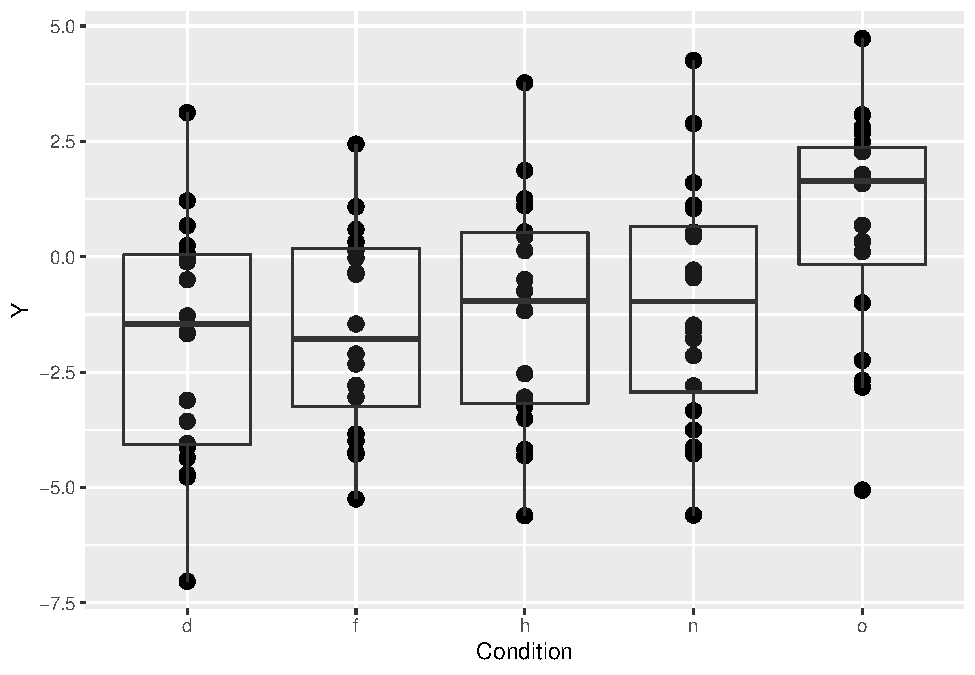
\includegraphics{perm_repeated_measures_files/figure-latex/unnamed-chunk-2-1.pdf}

Is there a specificity of the subject?

\begin{Shaded}
\begin{Highlighting}[]
\NormalTok{dati01}\OtherTok{=}\FunctionTok{subset}\NormalTok{(dati,Chan}\SpecialCharTok{==}\StringTok{"O1"}\NormalTok{)}
\FunctionTok{library}\NormalTok{(ggplot2)}
\NormalTok{p }\OtherTok{\textless{}{-}} \FunctionTok{ggplot}\NormalTok{(dati01,}\FunctionTok{aes}\NormalTok{(Condition,Y))}
\NormalTok{p}\SpecialCharTok{+}\FunctionTok{geom\_point}\NormalTok{(}\FunctionTok{aes}\NormalTok{(}\AttributeTok{group =}\NormalTok{ Subj, }\AttributeTok{colour =}\NormalTok{ Subj))}\SpecialCharTok{+}
  \FunctionTok{geom\_line}\NormalTok{(}\FunctionTok{aes}\NormalTok{(}\AttributeTok{group =}\NormalTok{ Subj, }\AttributeTok{colour =}\NormalTok{ Subj))}\SpecialCharTok{+}
   \FunctionTok{geom\_boxplot}\NormalTok{(}\AttributeTok{alpha=}\NormalTok{.}\DecValTok{1}\NormalTok{)}
\end{Highlighting}
\end{Shaded}

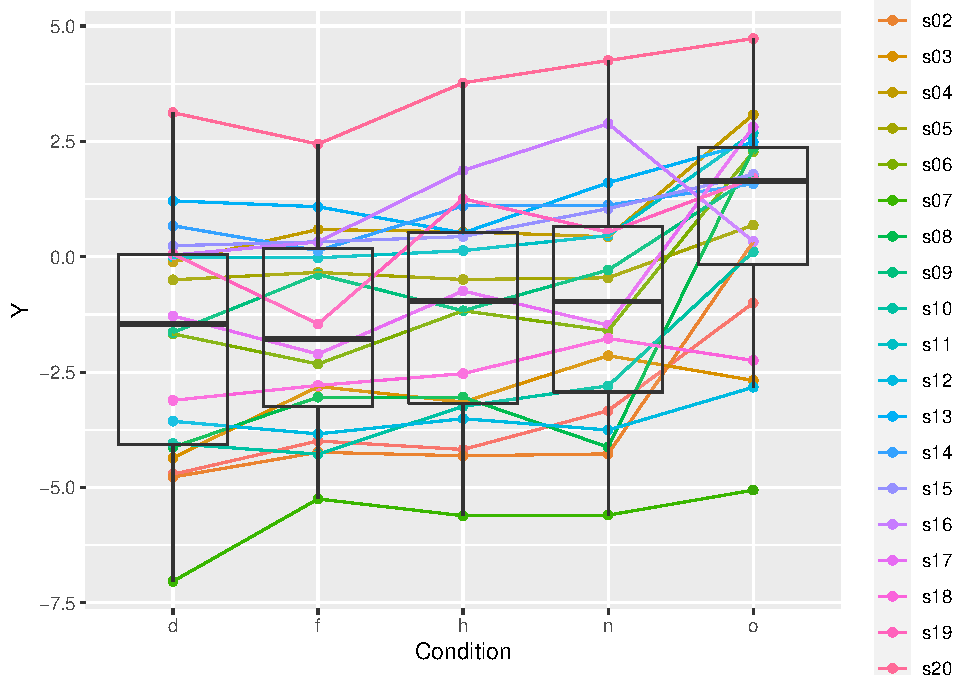
\includegraphics{perm_repeated_measures_files/figure-latex/unnamed-chunk-3-1.pdf}

We subtract the subject-specific effect (i.e.~subject's mean) to each
observation.

\begin{Shaded}
\begin{Highlighting}[]
\NormalTok{dati01}\OtherTok{=}\FunctionTok{subset}\NormalTok{(dati,Chan}\SpecialCharTok{==}\StringTok{"O1"}\NormalTok{)}
\NormalTok{Y}\OtherTok{=}\FunctionTok{scale}\NormalTok{(}\FunctionTok{matrix}\NormalTok{(dati01}\SpecialCharTok{$}\NormalTok{Y,}\DecValTok{5}\NormalTok{),}\AttributeTok{scale=}\ConstantTok{FALSE}\NormalTok{)}
\NormalTok{dati01}\SpecialCharTok{$}\NormalTok{Y}\OtherTok{=}\FunctionTok{as.vector}\NormalTok{(Y)}

\FunctionTok{library}\NormalTok{(ggplot2)}
\NormalTok{p }\OtherTok{\textless{}{-}} \FunctionTok{ggplot}\NormalTok{(dati01,}\FunctionTok{aes}\NormalTok{(Condition,Y))}
\NormalTok{p}\SpecialCharTok{+}\FunctionTok{geom\_point}\NormalTok{(}\FunctionTok{aes}\NormalTok{(}\AttributeTok{group =}\NormalTok{ Subj, }\AttributeTok{colour =}\NormalTok{ Subj))}\SpecialCharTok{+}
  \FunctionTok{geom\_line}\NormalTok{(}\FunctionTok{aes}\NormalTok{(}\AttributeTok{group =}\NormalTok{ Subj, }\AttributeTok{colour =}\NormalTok{ Subj))}\SpecialCharTok{+}
   \FunctionTok{geom\_boxplot}\NormalTok{(}\AttributeTok{alpha=}\NormalTok{.}\DecValTok{1}\NormalTok{)}
\end{Highlighting}
\end{Shaded}

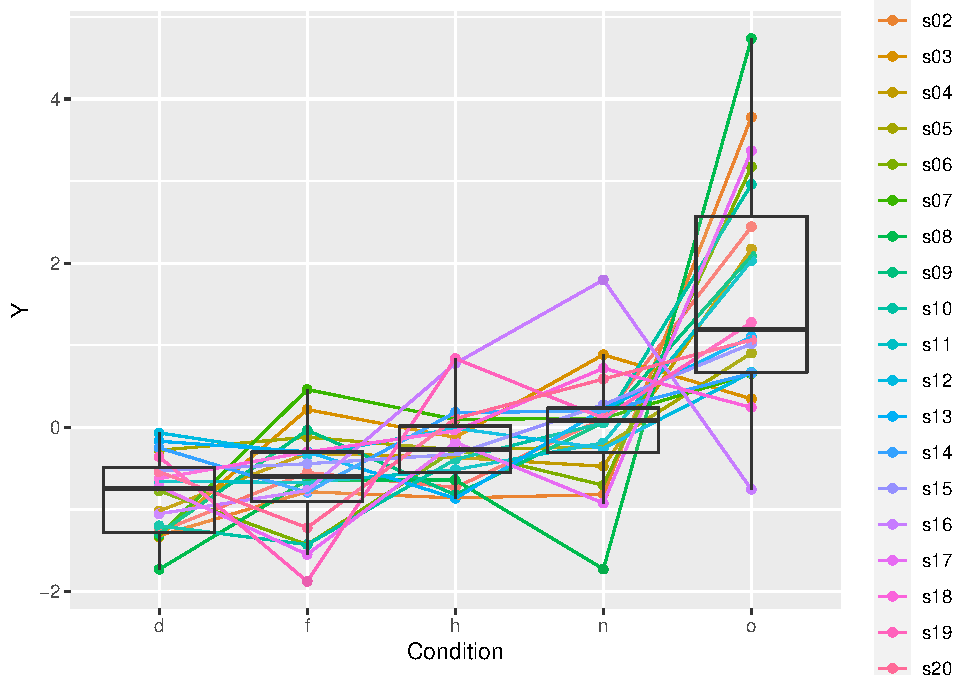
\includegraphics{perm_repeated_measures_files/figure-latex/unnamed-chunk-4-1.pdf}

The dispersion of the data has been largely reduced. This effect is the
one taken in account by the models for repeated measures.

\hypertarget{two-paired-samples-and-symmetry-test}{%
\section{Two Paired samples and symmetry
test}\label{two-paired-samples-and-symmetry-test}}

\hypertarget{definition}{%
\subsection{Definition}\label{definition}}

Let consider the reduced problem: channel \texttt{Chan=="O1} and
\texttt{Condition=="n"} or \texttt{Condition=="f"}.

Let be \(y\) the outcome, \(x\) the condition/treatment
(\(x\in \{1="f",2="n"\}\) in our case). Let be \(z=\) \texttt{Subject}
the nuisance factor in the stratified problem.

Under the null hypothesis: \(f(y|x=1,z)=f(y|x=2,z)=f(y|z)\)\\
while possibly (even under \(H_0\))
\(\exists (z,z'): f(y|x,z) \neq f(y|x',z')\)

This imply that observations are exchangeable only within the same
subject (\(z\), i.e.~playing the role of Strata).

In the gaussian-parametric approach we assume a different mean for each
subject (i.e.~Subject-specific effect), but the variance is forced to be
constant among subjects. Here we don't make this assumption. This is
much more realistic (see discussion later).

\hypertarget{testing-symmetry}{%
\subsection{Testing Symmetry}\label{testing-symmetry}}

The test statistic is based on the mean difference
\(T(y)=\sum_{i=1}^n (y_{i2}-y_{i1})/n=\sum_{i=1}^n d_{i}/n\)

Since \(f(y_{i1})=f(y|x=1,z=i)=f(y|x=2,z=i)=f(y_{i2})\), \(d_{i}\) is
symmetric.

Therefore, the null hypothesis is equivalentely written as:

\[
\begin{aligned}
H_0:&\ f(y_i|x_i=1,z_i)=f(y_i|x_i=2,z_i) \ \forall z_i \\
\implies & f(d_i)=f(-d_i)\ \forall z_i
\end{aligned}
\]

Permutantion within the observation \(i\) reduces to randomly flipping
the sign of \(d_i\). We test for symmetry.

\textbf{REMARK} The opposite implication is not always true:
\(f(d_i)=f(-d_i) \nRightarrow f(y_i|x_i=1,z_i)=f(y_i|x_i=2,z_i) \ \forall z_i\);
consider the important example of \(y_i\sim N(0,\Sigma(x_i,z_i))\)
(i.e.~the variance depends on the levels of \(x_i\) and the subject
\(z_i\)). In this case
\((y_i|x_i=1,z_i)-(y_i|x_i=2,z_i)\sim N(0,\Sigma(x_i=1,z_i)+\Sigma(x_i=2,z_i))\)
is still (normal and therefore) symmetric! Therefore the assumption of
symmetry of the difference is broader than the assumption of
exchangeability of observations within the same subject.

\hypertarget{a-bit-of-theory}{%
\subsection{A bit of theory}\label{a-bit-of-theory}}

(see also Pesarin, 2001; Hemerik \& Goeman, 2017)

Let \(Y\) be data taking values in a sample space \(\mathcal{Y}\). Let
\(\Pi\) be a finite set of transformations
\(\pi : \mathcal{Y} \rightarrow \mathcal{Y}\), such that \(\Pi\) is a
group with respect to the operation of composition of transformations:

\begin{itemize}
\tightlist
\item
  it contains identity,
\item
  every element has an inverse in the group,
\item
  closure: if \(\pi_1,\pi_2\in\Pi\): \(\pi_1\circ\pi_2\in\Pi\)
\end{itemize}

(e.g.~\(\Pi\) set of all possible permutations)

\textbf{Test statistic} \(T(Y):\ \mathbb{R}^n\to\mathbb{R}\)

\(H_0\): null hypothesis which implies that the joint distribution of
the test statistics \(T(\pi Y), \pi \in \Pi\), is invariant under all
transformations in \(\Pi\) of \(Y\). That is, writing
\(\Pi = \{\pi_1,\ldots, \pi_{|\Pi|}\}\), under \(H_0\):

\[T(\pi_1 Y), \ldots, T(\pi_{|\Pi|}Y) \overset{d}{=} T(\pi_1g Y), \ldots, T(\pi_{|\Pi|}gY)\]
for all \(g \in \Pi\).

Note that it holds when for all \(\pi \in \Pi\):
\(Y \overset{d}{=}\pi Y\).

\textbf{Orbit} of \(\mathcal{O}\):
\[\mathcal{O}=\{\pi Y : \pi \in \Pi\} \subseteq \mathcal{Y}\].

(losely) the set of all samples having the same likelihood under
\(H_0\).\\
\[\mathcal{O}=\{\pi \mathbf{y}:\ f(\pi \mathbf{y})=f(\mathbf{y}) \}\]
(\(|\mathcal{O}|\) number of elements of \(\mathcal{O}\))

If we assume exchangeability of observations, then:
\[\mathcal{O}=\{\textrm{all permutations of the observed data }\mathbf{y}\} = \{\mathbf{y}^*:\pi^*\circ\mathbf{y}\}\]

\textbf{Remark}: For Repeated Measures this means that, Under the Null
Hypothesis, observations within subject are assumed to be exchangeable:
\(f(y_1,y_2)=f(y_2,y_1)\).

This assumption is always true as long as observations:

\begin{itemize}
\tightlist
\item
  are \textbf{identically distributed} (within the same subject),\\
\item
  have the \textbf{same dependence}, e.g.~the same correlation.
\end{itemize}

\(t\)-test and linear models assumes independence, which is just a
special case: (\(f(y_1,y_2)=f(y_2)f(y_1)=f(y_2,y_1)\)), i.e.~a more
severe assumption!

paired \(t\)-test and repeated measures assumes homoscedasticity of the
vector of differences (i.e.~one difference for each subject), here we
only assume symmetry. Again, permutation approach makes less
assumptions.

\(T^{(k)}(Y)\) \(\lceil(1-\alpha)|\Pi|\ \rceil\)-th sorted value of
\(T(\pi Y)\)

\textbf{Theorem}: Under \(H_0\), \(P(T(Y) > T^{(k)}) \leq \alpha\).

intuition:

\[f(\mathbf{y}^*|\mathcal{O})=\frac{f(\mathbf{y}^*\cap\mathcal{O})}{f(\mathcal{O})}=
\frac{f(\mathbf{y}^*)}{f(\mathcal{O})}=
\frac{f(\mathbf{y}^*)}{f(\cup_{y\in\mathcal{O}}y)}=\frac{1}{|\mathcal{O}|}\ \forall\ \mathbf{y}^*\in \mathcal{O}\]
i.e.~each permutation is equally likely in the Orbit \(\mathcal{O}\).

(due to group structure) \[
\begin{aligned}
&P(T(\mathbf{y})\geq T^{(k)} | \mathbf{y}^*\in\mathcal{O}, H_0)=\\
&=\int_{T^{(k)}}^{+\infty} f(T(\mathbf{y}))dT(\mathbf{y})=\\
&=\sum_{\mathbf{y}\in\mathcal{O}} I(T(\mathbf{y}^*)\geq T(\mathbf{y}))/|\mathcal{O}|\leq \alpha
\ \ \ \ \forall\mathcal{O}
\end{aligned}
\]

\hypertarget{properties-see-pesarin-2001}{%
\subsubsection{Properties (see Pesarin,
2001)}\label{properties-see-pesarin-2001}}

The theorem above proves that the permutation tests have \textbf{exact
control of the type I error}, i.e.~\(P(p-value\leq \alpha|H_0)=\alpha\)
assuming \(\alpha\in \{1/|\mathcal{O}|,2/|\mathcal{O}|,\ldots,1\}\) -
don't forget that the orbit \(\mathcal{O}\) is a finite set; if this is
not the case, the test is (slightly) conservative.

Further properties:

\begin{itemize}
\tightlist
\item
  The permutations tests are \textbf{Unbiased}:
  \(P(p-value\leq \alpha|H_0)>\alpha\)\\
\item
  The test is \textbf{Consistent}: \(P(p-value\leq \alpha|H_1)\to 1\)
  when \(n\to\infty\)\\
\item
  The test converge to the parametric counterpart (when it exists)
\end{itemize}

\hypertarget{results}{%
\subsection{Results}\label{results}}

The parametric paired t-test:

\begin{Shaded}
\begin{Highlighting}[]
\FunctionTok{t.test}\NormalTok{(dati2}\SpecialCharTok{$}\NormalTok{Y[dati2}\SpecialCharTok{$}\NormalTok{Condition}\SpecialCharTok{==}\StringTok{"n"}\NormalTok{]}\SpecialCharTok{{-}}
\NormalTok{         dati2}\SpecialCharTok{$}\NormalTok{Y[dati2}\SpecialCharTok{$}\NormalTok{Condition}\SpecialCharTok{==}\StringTok{"f"}\NormalTok{])}
\end{Highlighting}
\end{Shaded}

\begin{verbatim}
## 
##  One Sample t-test
## 
## data:  dati2$Y[dati2$Condition == "n"] - dati2$Y[dati2$Condition == "f"]
## t = 3.287, df = 19, p-value = 0.003877
## alternative hypothesis: true mean is not equal to 0
## 95 percent confidence interval:
##  0.2303616 1.0380084
## sample estimates:
## mean of x 
##  0.634185
\end{verbatim}

The nonparametric one:

\begin{Shaded}
\begin{Highlighting}[]
\FunctionTok{flip}\NormalTok{(dati2}\SpecialCharTok{$}\NormalTok{Y[dati2}\SpecialCharTok{$}\NormalTok{Condition}\SpecialCharTok{==}\StringTok{"n"}\NormalTok{]}\SpecialCharTok{{-}}
\NormalTok{         dati2}\SpecialCharTok{$}\NormalTok{Y[dati2}\SpecialCharTok{$}\NormalTok{Condition}\SpecialCharTok{==}\StringTok{"f"}\NormalTok{],}\AttributeTok{perms=}\DecValTok{10000}\NormalTok{)}
\end{Highlighting}
\end{Shaded}

\begin{verbatim}
## 
##   Test  Stat tail p-value
## Y    t 3.287   ><  0.0038
\end{verbatim}

\begin{Shaded}
\begin{Highlighting}[]
\CommentTok{\# Equivalent to}
\FunctionTok{flip}\NormalTok{(Y}\SpecialCharTok{\textasciitilde{}}\NormalTok{Condition,}\AttributeTok{Strata=}\SpecialCharTok{\textasciitilde{}}\NormalTok{Subj,}\AttributeTok{data=}\NormalTok{dati2,}\AttributeTok{perms=}\DecValTok{10000}\NormalTok{)}
\end{Highlighting}
\end{Shaded}

\begin{verbatim}
## 
##   Test  Stat tail p-value
## Y    t 3.287   ><  0.0038
\end{verbatim}

\hypertarget{permutation-based-repeated-measures-anova}{%
\section{Permutation-Based Repeated Measures
ANOVA}\label{permutation-based-repeated-measures-anova}}

\hypertarget{introduction-1}{%
\subsection{Introduction}\label{introduction-1}}

Let be \(y\) the outcome, \(x\) the condition/treatment
(\(x\in (f,h,d,n,o)\) in our case). Let be \(z=\) \texttt{Subject} the
nuisance factor in a stratified problem.

Under the null hypothesis:
\(f(y|x,z)=f(y|x',z)=f(y|z) \ \forall (x,x')\)\\
while possibly (even under \(H_0\))
\(\exists (z,z'): f(y|x,z) \neq f(y|x',z')\)

This imply that observations are exchangeable only within the same
subject (\(z\)).

In the gaussian-parametric approach we assume a different mean for each
subject (i.e.~Subject-specific effect), but the variance is forced to be
constant among subjects. Here we don't make this assumption. This is
much more realistic (see discussion later).

\hypertarget{one-linear-model-for-each-subject}{%
\subsection{One Linear model for each
Subject}\label{one-linear-model-for-each-subject}}

The following approach is developed in Basso \& Finos (2012) and in
Finos \& Basso (2014). It is very similar to (basically an extension of)
the NonParametric Group level analysis developed in SnPM by Nichols and
Holmes (2001).

Assuming a hierarchical linear model we have a subject-specific linear
model for each subject. The vector of outcomes \(y_i\) can be modeled as
a linear function of the predictor

\(y_i=\beta_{0i}+\beta_{1i}x_1+\ldots+\beta_{ki}x_2+\varepsilon_i=X\beta_i+\varepsilon_i; \ i=1\ldots,n\)

\(y_i\) is a vector, \(X\) is a matrix of \(k\) predictors,
\(\varepsilon_i\) is a vector of iid r.v.

Therefore: \((\hat\beta_i|\beta_i)\sim (\beta_i,\Sigma_i)\)

We also assume that \(\beta_i\sim(\beta,\Psi)\). Therefore we have that:
\(\hat\beta_i\sim (\beta,\Psi+\Sigma_i)\)

Let's consider again the test on the effect of the Condition. The matrix
of predictors \(X\) is the matrix of \(k=C-1=4\) dummy variables. The
null hypothesis becomes: \[H_0: \beta=(\beta_1,\ldots,\beta_k)=0\] The
observations within the subject (i.e.~stratum) are exchangeable under
the null hypothesis. However, we don't have a \emph{separate} (in the
sense of Pesarin, 2001. This is often known as Subset Pivotality, WY,
1993) test for \(H_0:\beta_1=0\) since we are permuting the observation
under the global null hypothesis (i.e.~values relative to other
conditions affect the estimate of \(\beta_1\)).

The same problem rises if the matrix of \(X\) contains other factors,
such as \texttt{ChanL} and \texttt{Lateral}. Let's now consider the
experimental design modeled as a linear model with
\texttt{ChanL*Lateral*Condition}.

Data preparation:

\begin{Shaded}
\begin{Highlighting}[]
\NormalTok{dati}\SpecialCharTok{$}\NormalTok{Lateral}\OtherTok{=}\NormalTok{dati}\SpecialCharTok{$}\NormalTok{Chan}
\FunctionTok{levels}\NormalTok{(dati}\SpecialCharTok{$}\NormalTok{Lateral)}
\end{Highlighting}
\end{Shaded}

\begin{verbatim}
## [1] "O1"  "O2"  "P7"  "P8"  "PO7" "PO8"
\end{verbatim}

\begin{Shaded}
\begin{Highlighting}[]
\FunctionTok{levels}\NormalTok{(dati}\SpecialCharTok{$}\NormalTok{Lateral)[}\FunctionTok{c}\NormalTok{(}\DecValTok{1}\NormalTok{,}\DecValTok{3}\NormalTok{,}\DecValTok{5}\NormalTok{)]}\OtherTok{=}\StringTok{"Left"}
\FunctionTok{levels}\NormalTok{(dati}\SpecialCharTok{$}\NormalTok{Lateral)[}\SpecialCharTok{{-}}\DecValTok{1}\NormalTok{]}\OtherTok{=}\StringTok{"Right"}
\FunctionTok{levels}\NormalTok{(dati}\SpecialCharTok{$}\NormalTok{Lateral)}
\end{Highlighting}
\end{Shaded}

\begin{verbatim}
## [1] "Left"  "Right"
\end{verbatim}

\begin{Shaded}
\begin{Highlighting}[]
\NormalTok{dati}\SpecialCharTok{$}\NormalTok{ChanL}\OtherTok{=}\NormalTok{dati}\SpecialCharTok{$}\NormalTok{Chan}

\CommentTok{\# https://en.wikipedia.org/wiki/Regular\_expression}
\CommentTok{\# Digits: \textbackslash{}d}
\FunctionTok{levels}\NormalTok{(dati}\SpecialCharTok{$}\NormalTok{ChanL)}\OtherTok{=}\FunctionTok{gsub}\NormalTok{(}\StringTok{"}\SpecialCharTok{\textbackslash{}\textbackslash{}}\StringTok{d"}\NormalTok{,}\StringTok{""}\NormalTok{,}\FunctionTok{levels}\NormalTok{(dati}\SpecialCharTok{$}\NormalTok{ChanL))}

\FunctionTok{contrasts}\NormalTok{(dati}\SpecialCharTok{$}\NormalTok{Condition)}\OtherTok{=}\ConstantTok{NULL}
\FunctionTok{contrasts}\NormalTok{(dati}\SpecialCharTok{$}\NormalTok{ChanL)}\OtherTok{=}\ConstantTok{NULL}
\FunctionTok{contrasts}\NormalTok{(dati}\SpecialCharTok{$}\NormalTok{Lateral)}\OtherTok{=}\ConstantTok{NULL}
\end{Highlighting}
\end{Shaded}

We fit a model \emph{within} each subject and we store the vector of
estimated coefficients.

\begin{Shaded}
\begin{Highlighting}[]
\NormalTok{dataCoeff}\OtherTok{=}\FunctionTok{obs2coeffWithin}\NormalTok{(Y}\SpecialCharTok{\textasciitilde{}}\NormalTok{ ChanL}\SpecialCharTok{*}\NormalTok{Lateral}\SpecialCharTok{*}\NormalTok{Condition,}\AttributeTok{data=}\NormalTok{dati,}\AttributeTok{units=}\SpecialCharTok{\textasciitilde{}}\NormalTok{Subj)}
\end{Highlighting}
\end{Shaded}

From the results above we have that
\(\hat\beta_i\sim (\beta,\Psi+\Sigma_i)\). Since the model is full-rank
in this design (i.e.~no residuals error) and balanced, the distribution
is also symmetric around the mean:
\(f(\hat\beta_i-\beta)=f(-(\hat\beta_i-\beta))\) (at least
component-wise, i.e.~for marginal test)

We know, then, how to derive an exact test for \(H_0: \beta=0\). Now we
use these coefficients as a dataset to test for multivariate symmetry.

A very important result relies in the fact that the tests are separate,
that is, the symmetry under the null hypothesis is ensured for each
element of \(\beta\) whatever is the true mean of the others elements of
\(\beta\).

\begin{Shaded}
\begin{Highlighting}[]
\NormalTok{mod}\OtherTok{=}\FunctionTok{flipMixWithin}\NormalTok{(}\AttributeTok{data=}\NormalTok{dataCoeff,}\AttributeTok{perms=}\DecValTok{10000}\NormalTok{,}\AttributeTok{statTest =} \StringTok{"Tnaive"}\NormalTok{)}
\FunctionTok{summary}\NormalTok{(mod)}
\end{Highlighting}
\end{Shaded}

\begin{verbatim}
##  Call:
##  flipMixWithin(perms = 10000, data = dataCoeff, statTest = "Tnaive") 
## 9999 permutations.
## 
##                                        est.Su   Test    Stat tail p-value sig.
## (Intercept)_Tnaive                         NA Tnaive -3.1020   ><  0.0058   **
## ChanLP_Tnaive                              NA Tnaive -7.6164   ><  0.0002  ***
## ChanLPO_Tnaive                             NA Tnaive -5.2511   ><  0.0008  ***
## LateralRight_Tnaive                        NA Tnaive -1.7162   ><  0.0996     
## Conditionf_Tnaive                          NA Tnaive  0.9595   ><  0.3456     
## Conditionh_Tnaive                          NA Tnaive  4.8141   ><  0.0008  ***
## Conditionn_Tnaive                          NA Tnaive  4.5430   ><  0.0002  ***
## Conditiono_Tnaive                          NA Tnaive  6.7913   ><  0.0002  ***
## ChanLP:LateralRight_Tnaive                 NA Tnaive  0.5942   ><  0.5588     
## ChanLPO:LateralRight_Tnaive                NA Tnaive  2.4635   ><  0.0234    *
## ChanLP:Conditionf_Tnaive                   NA Tnaive -0.3815   ><  0.7118     
## ChanLPO:Conditionf_Tnaive                  NA Tnaive -0.7127   ><  0.4800     
## ChanLP:Conditionh_Tnaive                   NA Tnaive -1.2310   ><  0.2270     
## ChanLPO:Conditionh_Tnaive                  NA Tnaive -1.0945   ><  0.2850     
## ChanLP:Conditionn_Tnaive                   NA Tnaive  0.1750   ><  0.8640     
## ChanLPO:Conditionn_Tnaive                  NA Tnaive  0.2800   ><  0.7914     
## ChanLP:Conditiono_Tnaive                   NA Tnaive  4.5902   ><  0.0002  ***
## ChanLPO:Conditiono_Tnaive                  NA Tnaive  4.1505   ><  0.0014   **
## LateralRight:Conditionf_Tnaive             NA Tnaive  0.9319   ><  0.3518     
## LateralRight:Conditionh_Tnaive             NA Tnaive  0.1410   ><  0.8876     
## LateralRight:Conditionn_Tnaive             NA Tnaive  1.6669   ><  0.1138     
## LateralRight:Conditiono_Tnaive             NA Tnaive  0.5563   ><  0.5940     
## ChanLP:LateralRight:Conditionf_Tnaive      NA Tnaive -1.1426   ><  0.2640     
## ChanLPO:LateralRight:Conditionf_Tnaive     NA Tnaive -1.0363   ><  0.3134     
## ChanLP:LateralRight:Conditionh_Tnaive      NA Tnaive -0.5911   ><  0.5490     
## ChanLPO:LateralRight:Conditionh_Tnaive     NA Tnaive -2.1793   ><  0.0416    *
## ChanLP:LateralRight:Conditionn_Tnaive      NA Tnaive -0.6310   ><  0.5380     
## ChanLPO:LateralRight:Conditionn_Tnaive     NA Tnaive -1.4425   ><  0.1734     
## ChanLP:LateralRight:Conditiono_Tnaive      NA Tnaive  1.0884   ><  0.2860     
## ChanLPO:LateralRight:Conditiono_Tnaive     NA Tnaive -1.0263   ><  0.3234
\end{verbatim}

Since the fitted model within each subject is a saturated one, the
effect of each nuisance factor is removed without errors in the
estimates.

p-values for Global effect and factor are computed by NPC methodology.

\begin{Shaded}
\begin{Highlighting}[]
\CommentTok{\#Global}
\FunctionTok{npc}\NormalTok{(mod,}\AttributeTok{trace=}\ConstantTok{FALSE}\NormalTok{)}
\end{Highlighting}
\end{Shaded}

\begin{verbatim}
## 
##    comb.funct nVar  Stat p-value
## V1     Fisher   30 86.83  0.0002
\end{verbatim}

\begin{Shaded}
\begin{Highlighting}[]
\CommentTok{\# colnames(mod@permT)}
\CommentTok{\# Combined by factor}
\FunctionTok{summary}\NormalTok{(}\FunctionTok{npc}\NormalTok{(mod,}\AttributeTok{subsets =} \FunctionTok{list}\NormalTok{(}\AttributeTok{ChanL=}\DecValTok{1}\SpecialCharTok{:}\DecValTok{2}\NormalTok{,}\AttributeTok{Lateral=}\DecValTok{3}\NormalTok{,}\AttributeTok{Condition=}\DecValTok{4}\SpecialCharTok{:}\DecValTok{7}\NormalTok{,}
                       \AttributeTok{ChanL\_Lateral=}\DecValTok{8}\SpecialCharTok{:}\DecValTok{9}\NormalTok{,}
                       \AttributeTok{ChanL\_Condition=}\DecValTok{10}\SpecialCharTok{:}\DecValTok{17}\NormalTok{,}
                       \AttributeTok{Lateral\_Condition=}\DecValTok{18}\SpecialCharTok{:}\DecValTok{21}\NormalTok{,}
                       \AttributeTok{ChanL\_Lateral\_Condition=}\DecValTok{22}\SpecialCharTok{:}\DecValTok{29}\NormalTok{)))}
\end{Highlighting}
\end{Shaded}

\begin{verbatim}
##  Call:
##  npc(permTP = mod, subsets = list(ChanL = 1:2, Lateral = 3, Condition = 4:7,      ChanL_Lateral = 8:9, ChanL_Condition = 10:17, Lateral_Condition = 18:21,      ChanL_Lateral_Condition = 22:29)) 
##  permutations.
## 
##                         comb.funct nVar   Stat p-value sig.
## ChanL                       Fisher    2 13.667  0.0002  ***
## Lateral                     Fisher    1  7.131  0.0008  ***
## Condition                   Fisher    4 19.017  0.0004  ***
## ChanL_Lateral               Fisher    2  9.099  0.0004  ***
## ChanL_Condition             Fisher    8 16.464  0.0446    *
## Lateral_Condition           Fisher    4  9.909  0.0224    *
## ChanL_Lateral_Condition     Fisher    8 10.416  0.2074
\end{verbatim}

This approach is very general, it works also when we have non-balanced
and non-saturated models. For example we may like to use the values
computed on each single trial and not the average. In this case, the
model is not full rank and we have different number of trial in each
condition. In this case, the test remains exact only if we can assume
symmetric distribution of the errors. If this is not the case, the test
become approximated. It should be noted, however that usually the speed
in convergence to the exact control of the type I error is faster than
for parametric (gaussian) model since the our method becomes exact
whenever the distributions of the \(\hat\beta_i\) become symmetric
(i.e.~odd moments converge to zero), while the parametric one is exact
when the same distributions become normal (i.e.~both even and odd
moments converge to zero).

Furthermore, the symmetry is the only condition, we still allow for
hetheroscedastic errors between subjects. We also allow for different
design matrix between subjects (\(X_i\neq X_j\)). As an extreme and
surprisingly result, we also allow for the error within subject to
varies.

\hypertarget{comparison-with-parametric-mixed-model}{%
\subsection{Comparison with parametric
Mixed-Model}\label{comparison-with-parametric-mixed-model}}

Compare the previous results with the one of the parametric approach:

\begin{Shaded}
\begin{Highlighting}[]
\FunctionTok{library}\NormalTok{(lmerTest)}
\end{Highlighting}
\end{Shaded}

\begin{verbatim}
## Caricamento del pacchetto richiesto: lme4
\end{verbatim}

\begin{verbatim}
## Warning: il pacchetto 'lme4' è stato creato con R versione 4.1.2
\end{verbatim}

\begin{verbatim}
## Caricamento del pacchetto richiesto: Matrix
\end{verbatim}

\begin{verbatim}
## 
## Caricamento pacchetto: 'lmerTest'
\end{verbatim}

\begin{verbatim}
## Il seguente oggetto è mascherato da 'package:lme4':
## 
##     lmer
\end{verbatim}

\begin{verbatim}
## Il seguente oggetto è mascherato da 'package:stats':
## 
##     step
\end{verbatim}

\begin{Shaded}
\begin{Highlighting}[]
\NormalTok{mod\_mix}\OtherTok{=}\FunctionTok{lmer}\NormalTok{(Y}\SpecialCharTok{\textasciitilde{}}\NormalTok{ ChanL}\SpecialCharTok{*}\NormalTok{Lateral}\SpecialCharTok{*}\NormalTok{Condition }\SpecialCharTok{+}\NormalTok{(ChanL}\SpecialCharTok{*}\NormalTok{Lateral}\SpecialCharTok{|}\NormalTok{Subj),}\AttributeTok{data=}\NormalTok{dati)}

\NormalTok{car}\SpecialCharTok{::}\FunctionTok{Anova}\NormalTok{(mod\_mix)}
\end{Highlighting}
\end{Shaded}

\begin{verbatim}
## Analysis of Deviance Table (Type II Wald chisquare tests)
## 
## Response: Y
##                             Chisq Df Pr(>Chisq)    
## ChanL                     81.2681  2  < 2.2e-16 ***
## Lateral                    6.0196  1    0.01415 *  
## Condition               1200.8786  4  < 2.2e-16 ***
## ChanL:Lateral              7.7555  2    0.02070 *  
## ChanL:Condition           74.4535  8  6.346e-13 ***
## Lateral:Condition          0.8502  4    0.93160    
## ChanL:Lateral:Condition    2.8455  8    0.94367    
## ---
## Signif. codes:  0 '***' 0.001 '**' 0.01 '*' 0.05 '.' 0.1 ' ' 1
\end{verbatim}

The (parametric) Repeated measures method assumes of the errors, the
nonparametric (permutation) does not.

Mixed model does not make this assumption, but assumes normality and
homoscedasticity of the observations.

This could be a relevant point for our data:

\begin{Shaded}
\begin{Highlighting}[]
\NormalTok{dati}\SpecialCharTok{$}\NormalTok{residuals}\OtherTok{=}\FunctionTok{residuals}\NormalTok{(mod\_mix)}
\NormalTok{p }\OtherTok{\textless{}{-}} \FunctionTok{ggplot}\NormalTok{(dati, }\FunctionTok{aes}\NormalTok{(}\AttributeTok{x=}\NormalTok{Subj, }\AttributeTok{y=}\NormalTok{residuals,}\AttributeTok{fill=}\NormalTok{Condition)) }\SpecialCharTok{+}   \FunctionTok{geom\_boxplot}\NormalTok{()}
\NormalTok{p}
\end{Highlighting}
\end{Shaded}

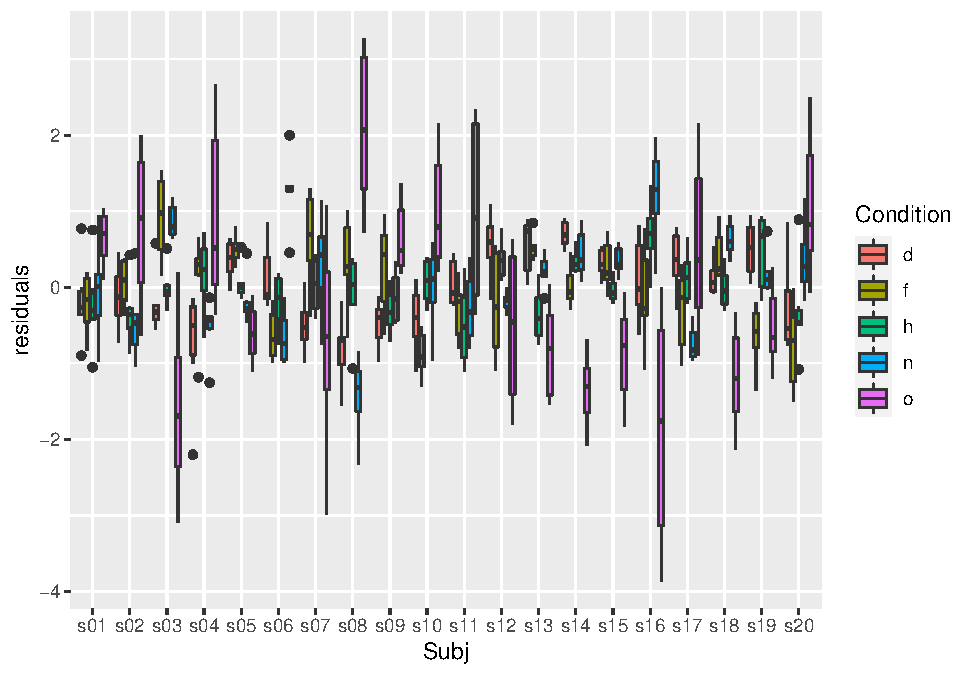
\includegraphics{perm_repeated_measures_files/figure-latex/unnamed-chunk-12-1.pdf}

The variability of the subjects doesn't not appear homogeneous.

\hypertarget{contrasts-and-post-hoc}{%
\subsection{Contrasts and post-hoc}\label{contrasts-and-post-hoc}}

\hypertarget{post-hoc-and-custom-contrasts}{%
\subsubsection{Post-hoc and Custom
contrasts}\label{post-hoc-and-custom-contrasts}}

For this example we restrict the analysis to the comparison
\texttt{Happy\ vs\ Neutral}.

Let' now compute the vectors of contrasts (one vector of reach channel,
length equal to number of subjects): \texttt{Happy\ vs\ Neutral}

\begin{Shaded}
\begin{Highlighting}[]
\FunctionTok{contrasts}\NormalTok{(dati}\SpecialCharTok{$}\NormalTok{Chan)}\OtherTok{=}\ConstantTok{NULL}
\FunctionTok{contrasts}\NormalTok{(dati}\SpecialCharTok{$}\NormalTok{Condition)}\OtherTok{=}\ConstantTok{NULL}

\NormalTok{dati\_2cond\_6chan}\OtherTok{=}\FunctionTok{subset}\NormalTok{(dati,(Condition}\SpecialCharTok{\%in\%}\FunctionTok{c}\NormalTok{(}\StringTok{"h"}\NormalTok{,}\StringTok{"n"}\NormalTok{)))}
\NormalTok{dati\_2cond\_6chan}\SpecialCharTok{$}\NormalTok{Condition}\OtherTok{=}\FunctionTok{factor}\NormalTok{(dati\_2cond\_6chan}\SpecialCharTok{$}\NormalTok{Condition)}
\NormalTok{dati\_2cond\_6chan}\SpecialCharTok{$}\NormalTok{Condition}\OtherTok{=}\FunctionTok{relevel}\NormalTok{(dati\_2cond\_6chan}\SpecialCharTok{$}\NormalTok{Condition,}\StringTok{"n"}\NormalTok{)}

\NormalTok{dataCoeff}\OtherTok{=}\FunctionTok{obs2coeffWithin}\NormalTok{(Y}\SpecialCharTok{\textasciitilde{}}\NormalTok{ Chan}\SpecialCharTok{*}\NormalTok{Condition,}\AttributeTok{data=}\NormalTok{dati\_2cond\_6chan,}\AttributeTok{units=}\SpecialCharTok{\textasciitilde{}}\NormalTok{Subj)}

\FunctionTok{colnames}\NormalTok{(dataCoeff}\SpecialCharTok{$}\NormalTok{coeffWithin)}
\end{Highlighting}
\end{Shaded}

\begin{verbatim}
##  [1] "(Intercept)"        "ChanO2"             "ChanP7"            
##  [4] "ChanP8"             "ChanPO7"            "ChanPO8"           
##  [7] "Conditionh"         "ChanO2:Conditionh"  "ChanP7:Conditionh" 
## [10] "ChanP8:Conditionh"  "ChanPO7:Conditionh" "ChanPO8:Conditionh"
\end{verbatim}

\texttt{dataCoeff\$coeffWithin} contains the estimates of the
coefficients for the model for each subject.

The column \texttt{Conditionh} contains the contrast \texttt{h-n} in
\texttt{Chan01}. To get the same contrast in any other channel we add
the column of interaction \texttt{Conditionh:Chan} to the one of
\texttt{Chan01}. As an example, to get \texttt{n-f} in \texttt{Chan02}
we make \texttt{Conditionh\ +\ ChanO2:Conditionh}.

\begin{Shaded}
\begin{Highlighting}[]
\NormalTok{Y}\OtherTok{=}\NormalTok{dataCoeff}\SpecialCharTok{$}\NormalTok{coeffWithin[,}\DecValTok{7}\NormalTok{]}\SpecialCharTok{+}\FunctionTok{cbind}\NormalTok{(}\AttributeTok{ChanO1=}\DecValTok{0}\NormalTok{,dataCoeff}\SpecialCharTok{$}\NormalTok{coeffWithin[,}\DecValTok{8}\SpecialCharTok{:}\DecValTok{12}\NormalTok{])}
\FunctionTok{colnames}\NormalTok{(Y)}\OtherTok{=}\FunctionTok{gsub}\NormalTok{(}\StringTok{":Condition."}\NormalTok{,}\StringTok{""}\NormalTok{,}\FunctionTok{colnames}\NormalTok{(Y))}
\FunctionTok{colnames}\NormalTok{(Y)}
\end{Highlighting}
\end{Shaded}

\begin{verbatim}
## [1] "ChanO1"  "ChanO2"  "ChanP7"  "ChanP8"  "ChanPO7" "ChanPO8"
\end{verbatim}

Analysis: raw and adjusted p-values (min-p procedure)

\begin{Shaded}
\begin{Highlighting}[]
\NormalTok{res}\OtherTok{=}\FunctionTok{flip}\NormalTok{(Y,}\AttributeTok{perms=}\DecValTok{10000}\NormalTok{)}

\NormalTok{res}\OtherTok{=}\FunctionTok{flip.adjust}\NormalTok{(res)}
\FunctionTok{summary}\NormalTok{(res)}
\end{Highlighting}
\end{Shaded}

\begin{verbatim}
##  Call:
##  flip(Y = Y, perms = 10000) 
## 9999 permutations.
## 
##         Test   Stat tail p-value Adjust:maxT sig.
## ChanO1     t -1.472   ><  0.1594      0.1594     
## ChanO2     t -2.137   ><  0.0438      0.0744     
## ChanP7     t -2.449   ><  0.0264      0.0588     
## ChanP8     t -3.675   ><  0.0022      0.0056   **
## ChanPO7    t -2.375   ><  0.0322      0.0620     
## ChanPO8    t -2.981   ><  0.0060      0.0212    *
\end{verbatim}

To show the results plot intensity colors based on the significance of
the adjusted p-values for each channel. Just for visual purposes, we
transform the adjusted p-values by \(-log10(p)\):

\begin{Shaded}
\begin{Highlighting}[]
\CommentTok{\# install.packages("legit")}
\FunctionTok{library}\NormalTok{(eegkit)}
\end{Highlighting}
\end{Shaded}

\begin{verbatim}
## Warning: il pacchetto 'eegkit' è stato creato con R versione 4.1.3
\end{verbatim}

\begin{verbatim}
## Warning: il pacchetto 'rgl' è stato creato con R versione 4.1.2
\end{verbatim}

\begin{Shaded}
\begin{Highlighting}[]
\CommentTok{\# get the a z value from the adjusted p{-}value for each channel, just for visual purposes:}
\NormalTok{pvals}\OtherTok{=}\FunctionTok{getFlip}\NormalTok{(res,}\StringTok{"Adjust:maxT"}\NormalTok{)}
\FunctionTok{rownames}\NormalTok{(pvals)}\OtherTok{=}\FunctionTok{gsub}\NormalTok{(}\StringTok{"Chan"}\NormalTok{,}\StringTok{""}\NormalTok{,}\FunctionTok{rownames}\NormalTok{(pvals))}

\CommentTok{\# match to eeg coordinates}
\FunctionTok{data}\NormalTok{(eegcoord)}
\NormalTok{cidx }\OtherTok{\textless{}{-}} \FunctionTok{match}\NormalTok{(}\FunctionTok{rownames}\NormalTok{(pvals),}\FunctionTok{rownames}\NormalTok{(eegcoord))}

\CommentTok{\# plot t{-}stat in 2d}
\FunctionTok{eegspace}\NormalTok{(eegcoord[cidx,}\DecValTok{4}\SpecialCharTok{:}\DecValTok{5}\NormalTok{],}\SpecialCharTok{{-}}\FunctionTok{log10}\NormalTok{(pvals[,}\DecValTok{1}\NormalTok{]),}\AttributeTok{cex.point =} \DecValTok{3}\NormalTok{,}\AttributeTok{colorlab=}\StringTok{"{-}log10(adj{-}p)"}\NormalTok{,}\AttributeTok{mycolors=}\FunctionTok{heat.colors}\NormalTok{(}\DecValTok{4}\NormalTok{))}
\end{Highlighting}
\end{Shaded}

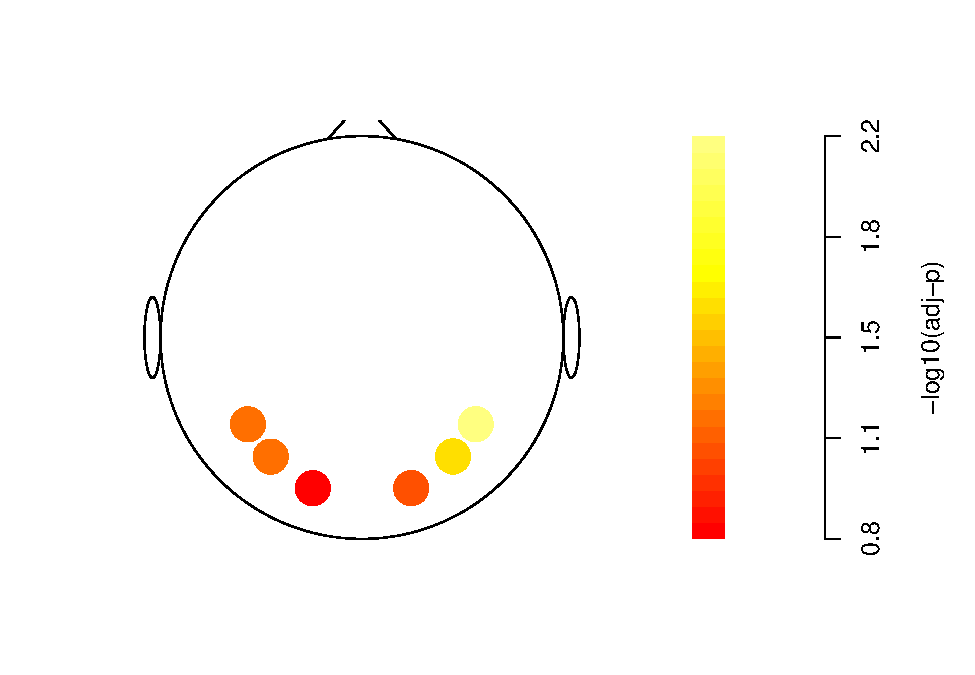
\includegraphics{perm_repeated_measures_files/figure-latex/unnamed-chunk-16-1.pdf}

\hypertarget{minimal-bibliography}{%
\section{(minimal) Bibliography}\label{minimal-bibliography}}

\begin{itemize}
\item
  Basso \& Finos (2012). Exact Multivariate Permutation Tests for Fixed
  Effects in Mixed-Models. \emph{Communications in Statistics - Theory
  and Methods}, 41: 2991 - 3001.
\item
  Finos \& Basso (2014) Permutation tests for between-unit fixed effects
  in multivariate generalized linear mixed models. \emph{Stat Comput}
  24, 941--952.
\item
  Nichols \& Holmes (2001) Nonparametric Permutation Tests For
  Functional Neuroimaging: A Primer with Examples. \emph{Human Brain
  Mapping} 15, 1-25.
  \url{https://onlinelibrary.wiley.com/doi/ftr/10.1002/hbm.1058}
\end{itemize}

\end{document}
